% 18-09-2024

\chapter{Espacios Topológicos}

\begin{definicion}
    Un \textbf{espacio topológico} es una par $(X, \cc{T})$, donde $X \neq \emptyset$ es un conjunto y $\cc{T}\subset\cc{P}(X)$ es una familia de subconjuntos de $X$.

    \begin{enumerate}
        \item[\textbf{(\hypertarget{A1}{A1})}] $\emptyset, X \in \cc{T}$.
        \item[\textbf{(\hypertarget{A2}{A2})}] Si $\{U_i\}_{i\in I} \subset \cc{T}$, entonces $\bigcup\limits_{i\in I} U_i \in \cc{T}$.
        \item[\textbf{(\hypertarget{A3}{A3})}] Si $U_1, U_2 \in \cc{T}$, entonces $U_1 \cap U_2 \in \cc{T}$.
    \end{enumerate}

    A la familia $\cc{T}$ se le llama \textbf{topología} en el conjunto $X$. A los elementos de $\cc{T}$ se les llama \textbf{abiertos} en el espacio topológico $(X, \cc{T})$.
\end{definicion}

\vspace*{0.5cm}

\begin{observacion}
    De \hyperlink{A1}{\textbf{(A1)}} podemos concretar que si $U_1, \dots, U_k \in \cc{T}$, entonces \smash{$\bigcap\limits_{i=1}^{\infty}U_i \in \cc{T}$}.
    En general, si $\{U_i\}_{i=1}^{\infty}\in \cc{T}$, entonces $\bigcup\limits_{i=1}^{\infty}$ no tiene por qué ser abierto.
\end{observacion}

\begin{ejemplo}\ 
    \begin{itemize}
        \item \textbf{Topología trivial:} Sea $X \neq \emptyset$, $\cc{T}_t = \{\emptyset, X\} \Rightarrow (X, \cc{T}_t)$ es un e.t\footnote{A partir de ahora notaremos así a un espacio topológico}.
        \item \textbf{Topología discreta:} Sea $X \neq \emptyset$, $\cc{T}_{disc}= \cc{T}_{D} = \cc{P}(X) \Rightarrow (X, \cc{T}_D)$ es un e.t.
        \item \textbf{Topología del punto incluido:} Sea $X \neq \emptyset$, $x_0\in X$ $\cc{T}_{x_0} = \{\emptyset\}\cup \{U \subset X : x_0 \in U\} \Rightarrow (X, \cc{T}_{x_0})$ es un e.t.
        \item \textbf{Topología cofinita:} (o topología de los complementos finitos) Sea $X \neq \emptyset$, $\cc{T}_{CF} = \{\emptyset\}\cup\{U\subset X : X \setminus U \text{ es finito}\} \Rightarrow (X, \cc{T}_{CF})$ es un e.t.
        \begin{gather*}
            X \setminus \left(\bigcup\limits_{i\in I}U_i\right) = \bigcap\limits_{i\in I}(X \setminus U_i) \text{(intersección de finitos es finito)}\\
            X \setminus (U_1 \cap U_2) = (X\setminus U_1) \cup (X \setminus U_2)\text{(unión de finitos es finito)}
        \end{gather*}
        \item \textbf{Topología conumerable:} (o topología de los complementos numerables) Sea $X \neq \emptyset$, $\cc{T}_{CF} = \{\emptyset\}\cup\{U\subset X : X \setminus U \text{ es numerable}\} \Rightarrow (X, \cc{T}_{CF})$ es un e.t.
        \item $\bb{R}$, $ \cc{T}=\{\emptyset, \bb{R}, \bb{Q}, \bb{R}\setminus \bb{Q}\}, \Rightarrow (\bb{R}, \cc{T})$ es un e.t. 
        \item \textbf{Topología de Sierpinski:} $X=\{a,b\}$, $\cc{T}=\{\emptyset, \{a\}, X\} \Rightarrow (X, \cc{T})$ es un e.t.
        \item \textbf{Topología de Sorgenfrey:} $X=\bb{R}$, $\cc{T}_S$, $U\in \cc{T}_S \sii \forall x \in U \ \  \exists \veps > 0 \text{ tal que } [x, x+\veps) \subset U$. (es un caso particular del punto incluido, $\cc{T}_a$).
    \end{itemize}

    \newpage

    \begin{observacion}
        En $X=\{x\}$ solo existe una topología, $\cc{T}=\{\emptyset, \{x\}\}$ (todas las topologías son la misma).
    \end{observacion}

    \begin{ejercicio}
        Determinar todas las topologías en un conjunto con 2 elementos.\\
        % Hay 4: trivial, discreta y punto incluido con cada elemento

        Consideramos $X=\{a,b\}$. Las topologías posibles son:
        \begin{itemize}
            \item Trivial: $\cc{T}_t=\{\emptyset, X\}$
            \item Discreta: $\cc{T}_{disc}=\cc{P}(X)$
            \item Punto incluido (a): $\cc{T}_a = \{\emptyset, \{a\}, X\}$
            \item Punto incluido (b): $\cc{T}_b = \{\emptyset, \{b\}, X\}$
        \end{itemize}
        \endsquare
    \end{ejercicio}

    \begin{ejercicio}
        Sea $(X, \cc{T})$ e.t. Demostrar que $\cc{T}=\cc{T}_{disc} \sii \{x\}\in \cc{T}\ \  \forall x \in X$. 
        % Implicación derecha es trivial
        \begin{itemize}
            \item[$\Rightarrow$)] Si $\cc{T} = \cc{T}_{disc}$, como $\{x\}\in \cc{P}(X) \ \ \forall x \in X$, se tiene que $\{x\}\in \cc{T}_{disc} = \cc{T}$.
            \item[$\Leftarrow$)] Tenemos $\{x\} \in \cc{T} \ \ \forall x \in X$. Consideramos $U \in \cc{P}(X)$ un subconjunto cualquiera de $X$. Podemos expresar $U=\bigcup\limits_{i\in I} \{x_i\}$, donde $\{x_i\} \in X \ \ \forall i \in I$. Por la propiedad \apuntar{A2} tenemos $U \in \cc{T}$. Como $U$ era un subconjunto arbitrario de $X$, tenemos $\cc{T}=\cc{T}_{disc}$.
        \end{itemize}
        \endsquare
    \end{ejercicio}

    \section{Topología métrica. La topología usual de $\bb{R}^n$}

    \begin{definicion}
        Un \textbf{espacio métrico} es un par $(X, d)$ donde $X \neq \emptyset$ es un conjunto y $d: X \times X \rightarrow \bb{R}$ es una aplicación que verifica:
    \end{definicion}

    \begin{enumerate}
        \item [\textbf{(\hypertarget{D1}{D1})}] $d(x, y) \geq 0$\ \ $\forall x,y \in X$. Además, $d(x,y)= 0 \sii x=y$.
        \item [\textbf{(\hypertarget{D2}{D2})}] (simetría) $d(x,y)=d(y,x)$ $\forall x, y, \in X.$
        \item [\textbf{(\hypertarget{D3}{D3})}] (desigualdad triangular) $d(x,z) \leq d(x,y) + d(y,z)$\ \ $\forall x,y,z \in X$
    \end{enumerate}

    A la aplicación $d$ la llamaremos \textbf{distancia}.

    \begin{ejercicio}
        % (D2) + (D3) + 2ª parte de (D1) se deduce 1ª parte de (D1) luego $d:X \times X \rightarrow [0, \infty)$
        Demostrar que a partir de las propiedades \hyperlink{D2}{\textbf{(D2)}}, \hyperlink{D3}{\textbf{(D3)}} y la segunda parte de \hyperlink{D1}{\textbf{(D1)}} se puede deducir la primera parte de \hyperlink{D1}{\textbf{(D1)}}, y como consecuencia se tiene $d:X \times X \rightarrow [0, \infty)$.\\

        Para cualesquiera $x,y \in X$, tenemos:
        \begin{gather*}
            0 \overset{\apuntar{D1}{(2)}}{=} d(x,x) \overset{\apuntar{D3}}{\leq} d(x,y) + d(y,x) \overset{\apuntar{D2}}{=} d(x,y) + d(x,y) = 2 d(x,y)
        \end{gather*}
        De donde podemos deducir
        \begin{gather*}
            d(x,y) \geq 0 \Rightarrow d:X \times X \rightarrow [0, \infty)
        \end{gather*}

        \endsquare
         
    \end{ejercicio}

   \begin{definicion}
        $(X,d)$ e.m. $x \in X$, $r >0$, se definen:

        \begin{itemize}
            \item La \textbf{bola (abierta)} de centro $x$ y radio $r$ como 
            \begin{gather*}
                B(x, r) = \{y \in X : d(x,y) < r\} \subset X
            \end{gather*}
            \item La \textbf{bola cerrada} de centro $x$ y radio $r$ como 
            \begin{gather*}
                \overline{B}(x, r) = \{y \in X : d(x,y) \leq r\} \subset X
            \end{gather*}
            \item La \textbf{esfera} de centro $x$ y radio $r$ como 
            \begin{gather*}
                S(x, r) = \{y \in X : d(x,y) = r\} \subset X
            \end{gather*}
        \end{itemize}
   \end{definicion}

    Algunas propiedades que se deducen de la definición anterior son:
    \begin{itemize}
        \item $\overline{B}(x, r) = B(x,r) \cup S(x,r)$
        \item $S(x,r) = \overline{B}(x, r) \setminus B(x,r)$
        \item Si $s<r$, entonces $\overline{B}(x, x) \subset B(x,r)$
    \end{itemize}

    \begin{ejemplo}(Espacio euclídeo $\bb{R}^n$)
        En $\bb{R}^n$ consideramos la \textbf{distancia usual}, 
        \begin{gather*}
            d(x,y) = \|x-y\| = \sqrt{\sum\limits_{i=1}^2(x_i-y_i)^2}
        \end{gather*}

        Al espacio métrico $(\bb{R}^n, d )$ lo denominaremos \textbf{Espacio Euclídeo}.

        \begin{itemize}
            \item Si $n=1$, $d(x,y) = |x-y|$,,  %Arreglar
            \begin{align*}
                B(x,r) &= (x-r, x+r)\\
                \overline{B}(x,r) &= [x-r, x+r]\\
                S(x,r) &= \{x,y\}
            \end{align*}
            
            \item En $n=2$ tenemos
            
            \vspace*{0.25cm}

            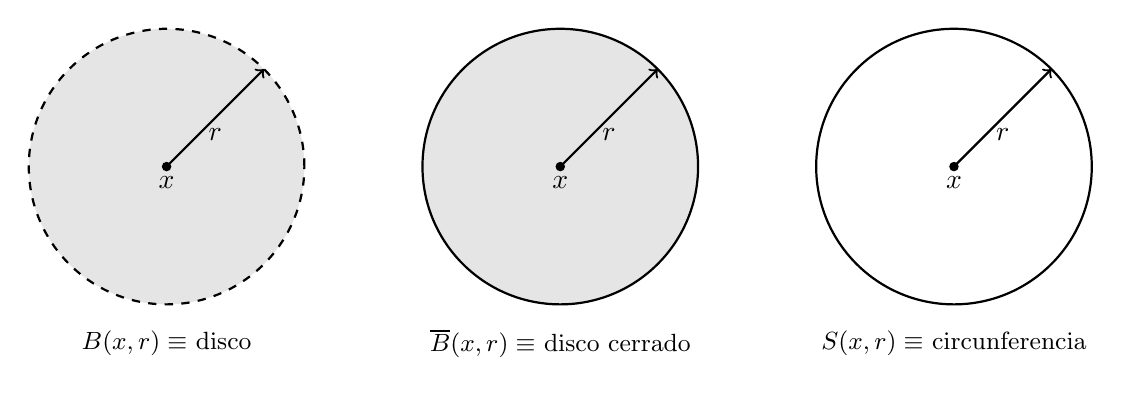
\begin{tikzpicture}
                \centering

                \def\radius{1.75}
                \def\incolor{gray!20}
                \def\angulo{45}

                % Desactiva los caracteres conflictivos
                \shorthandoff{>} % Para poner puntas de flecha

                \filldraw[dashed, fill=\incolor, thick] (-5,0) circle (\radius);
                \filldraw (-5,0) circle (1.5pt)  node[below] {$x$};
                \draw[thick, ->] (-5,0) -> ({-5+sin(\angulo)*\radius}, {cos(\angulo)*\radius}) node[midway, below] {$r$};
                \node at (-5,-2.25) {\small{$B(x,r) \equiv$ disco}};

                \filldraw[fill=\incolor, thick] (0,0) circle (\radius);
                \filldraw (0,0) circle (1.5pt)  node[below] {$x$};
                \draw[thick, ->] (0,0) -> ({sin(\angulo)*\radius}, {cos(\angulo)*\radius}) node[midway, below] {$r$};
                \node at (0,-2.25) {\small{$\overline{B}(x,r) \equiv$ disco cerrado}};

                \draw[thick] (5,0) circle (\radius);
                \filldraw (5,0) circle (1.5pt)  node[below] {$x$};
                \draw[thick, ->] (5,0) -> ({5+sin(\angulo)*\radius}, {cos(\angulo)*\radius}) node[midway, below] {$r$};
                \node at (5,-2.25) {\small{$S(x,r) \equiv$ circunferencia}};
            \end{tikzpicture}

            \item En $n=3$ tenemos:
            
            \vspace*{0.25cm}

            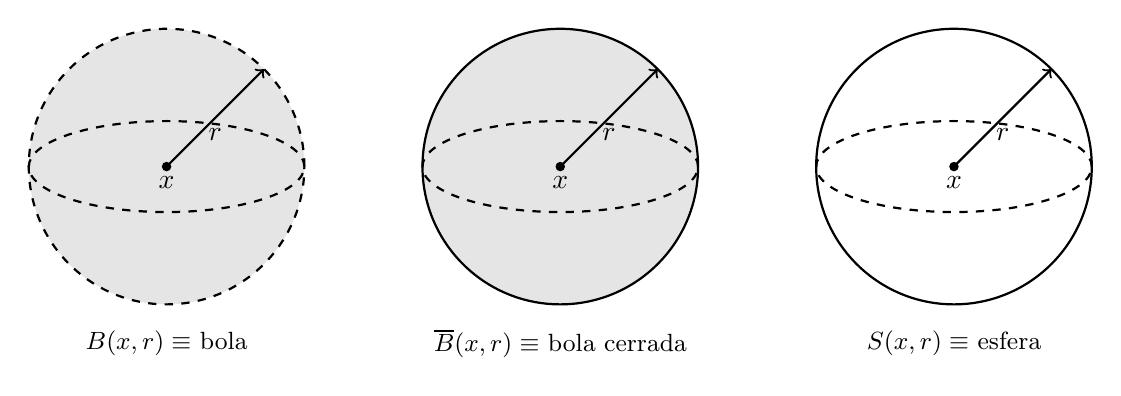
\begin{tikzpicture}
                \centering

                \def\radius{1.75}
                \def\incolor{gray!20}
                \def\angulo{45}

                % Desactiva los caracteres conflictivos
                \shorthandoff{>} % Para poner puntas de flecha

                \filldraw[dashed, fill=\incolor, thick] (-5,0) circle (\radius);
                \draw[dashed, thick] (-5,0) ellipse [x radius=\radius, y radius=0.33*\radius];
                \filldraw (-5,0) circle (1.5pt)  node[below] {$x$};
                \draw[thick, ->] (-5,0) -> ({-5+sin(\angulo)*\radius}, {cos(\angulo)*\radius}) node[midway, below] {$r$};
                \node at (-5,-2.25) {\small{$B(x,r) \equiv$ bola}};

                \filldraw[fill=\incolor, thick] (0,0) circle (\radius);
                \draw[dashed, thick] (0,0) ellipse [x radius=\radius, y radius=0.33*\radius];
                \filldraw (0,0) circle (1.5pt)  node[below] {$x$};
                \draw[thick, ->] (0,0) -> ({sin(\angulo)*\radius}, {cos(\angulo)*\radius}) node[midway, below] {$r$};
                \node at (0,-2.25) {\small{$\overline{B}(x,r) \equiv$ bola cerrada}};

                \draw[thick] (5,0) circle (\radius);
                \draw[dashed, thick] (5,0) ellipse [x radius=\radius, y radius=0.33*\radius];
                \filldraw (5,0) circle (1.5pt)  node[below] {$x$};
                \draw[thick, ->] (5,0) -> ({5+sin(\angulo)*\radius}, {cos(\angulo)*\radius}) node[midway, below] {$r$};
                \node at (5,-2.25) {\small{$S(x,r) \equiv$ esfera}};
            \end{tikzpicture}
        \end{itemize}
    \end{ejemplo}

    \begin{ejemplo}
        $X \neq \emptyset$ se define la \textbf{distancia discreta} como 
        \begin{align*}
            d_{disc}(x,y) &=
            \left\{ 
            \begin{array}{ccc}
                0 & \text{si} & x=y\\
                1 & \text{si} & x\neq y
            \end{array}
            \right. 
        \end{align*}
        Con la distancia así definida tenemos:
        \begin{align*}
            B(x,y) &=
            \left\{ 
            \begin{array}{ccc}
                X & \text{si} & r>1\\
                \{x\} & \text{si} & r \leq 1
            \end{array}
            \right. \\\\
            \overline{B}(x,y) &=
            \left\{ 
            \begin{array}{ccc}
                X & \text{si} & r \geq 1\\
                \{x\} & \text{si} & r < 1
            \end{array}
            \right.\\\\
            S(x,y) &=
            \left\{ 
            \begin{array}{ccc}
                X \setminus \{x\} & \text{si} & r =1 \\
                \emptyset & \text{si} & r \neq 1\\
            \end{array}
            \right.
        \end{align*}
    \end{ejemplo}

    Tu escribes aq normal y te va saliendo.

\end{ejemplo}


